%!TEX root = ../report.tex

%
% Architecture
%

\section{Architecture} % (fold)
\label{sec:architecture}

This work will follow the architecture described in Figure~\ref{fig:architecture}.
There will be a module in Racket that will provide a Racket interface for the rest of the system using \emph{Racket FFI} and is through this that the users will mostly interact with the system. This will be a layer that will not have an impact on performance. 


\begin{wrapfigure}{r}{0.5\textwidth}
	\vspace{-15pt}
    \centering
	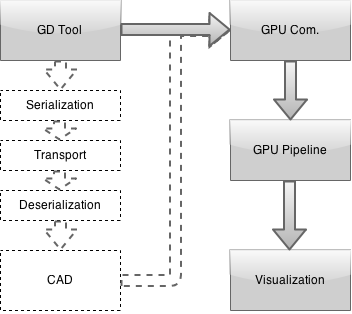
\includegraphics[width=0.5\textwidth]{img/Architecture/GD-Fast-Pipeline.png}
	\caption{High Level Architecture}
	\label{fig:architecture}
	\vspace{-15pt}
\end{wrapfigure}

The second step is the OpenGL layer, that implement the Racket interface and than create the window and manage user input. The functions provided to Racket will create here the description of the geometry that will be \emph{amplified} in the next phase. This description is one $GL\_POINT$ per geometric primitive that represent the position of that primitive and it is also embedded with an array of floats that encode the type of geometry and specific information like size or number of sides.

In the last step are the shaders, where most of the work is done. This receives the small description of the geometry and generates the primitives to be drawn. To achieve this, it is applied the concept of geometry amplification. As told in Section~\ref{sub:geometriy_shaders}, this method has limitations that could make an impact on how the geometry generation is implemented. However OpenGL guarantee support for at least 256 vertices which is enough to generate the majority of geometric primitives. Since this problem is hardware dependent and GPU hardware are getting more powerful I believe that this will not be a problem in the near future.

This architecture significantly reduces the amount of data that is moved between layers and takes advantage of the power that recent GPUs have.

For instance the following code results in the Figure~\ref{fig:pic1} that is a procedural generated model of a city with ~40k buildings. This example was generated with the current prototype with the following Racket code:

\begin{lstlisting}[frame=single,language=Lisp]
(init 0)
(city 100)
(start)
\end{lstlisting}

The \emph{init} command makes an initialization of the system, the \emph{start} command starts creates the window and starts the visualization. In between the model is created, in this case with the function city.

\begin{figure}[htb]
	\centering
	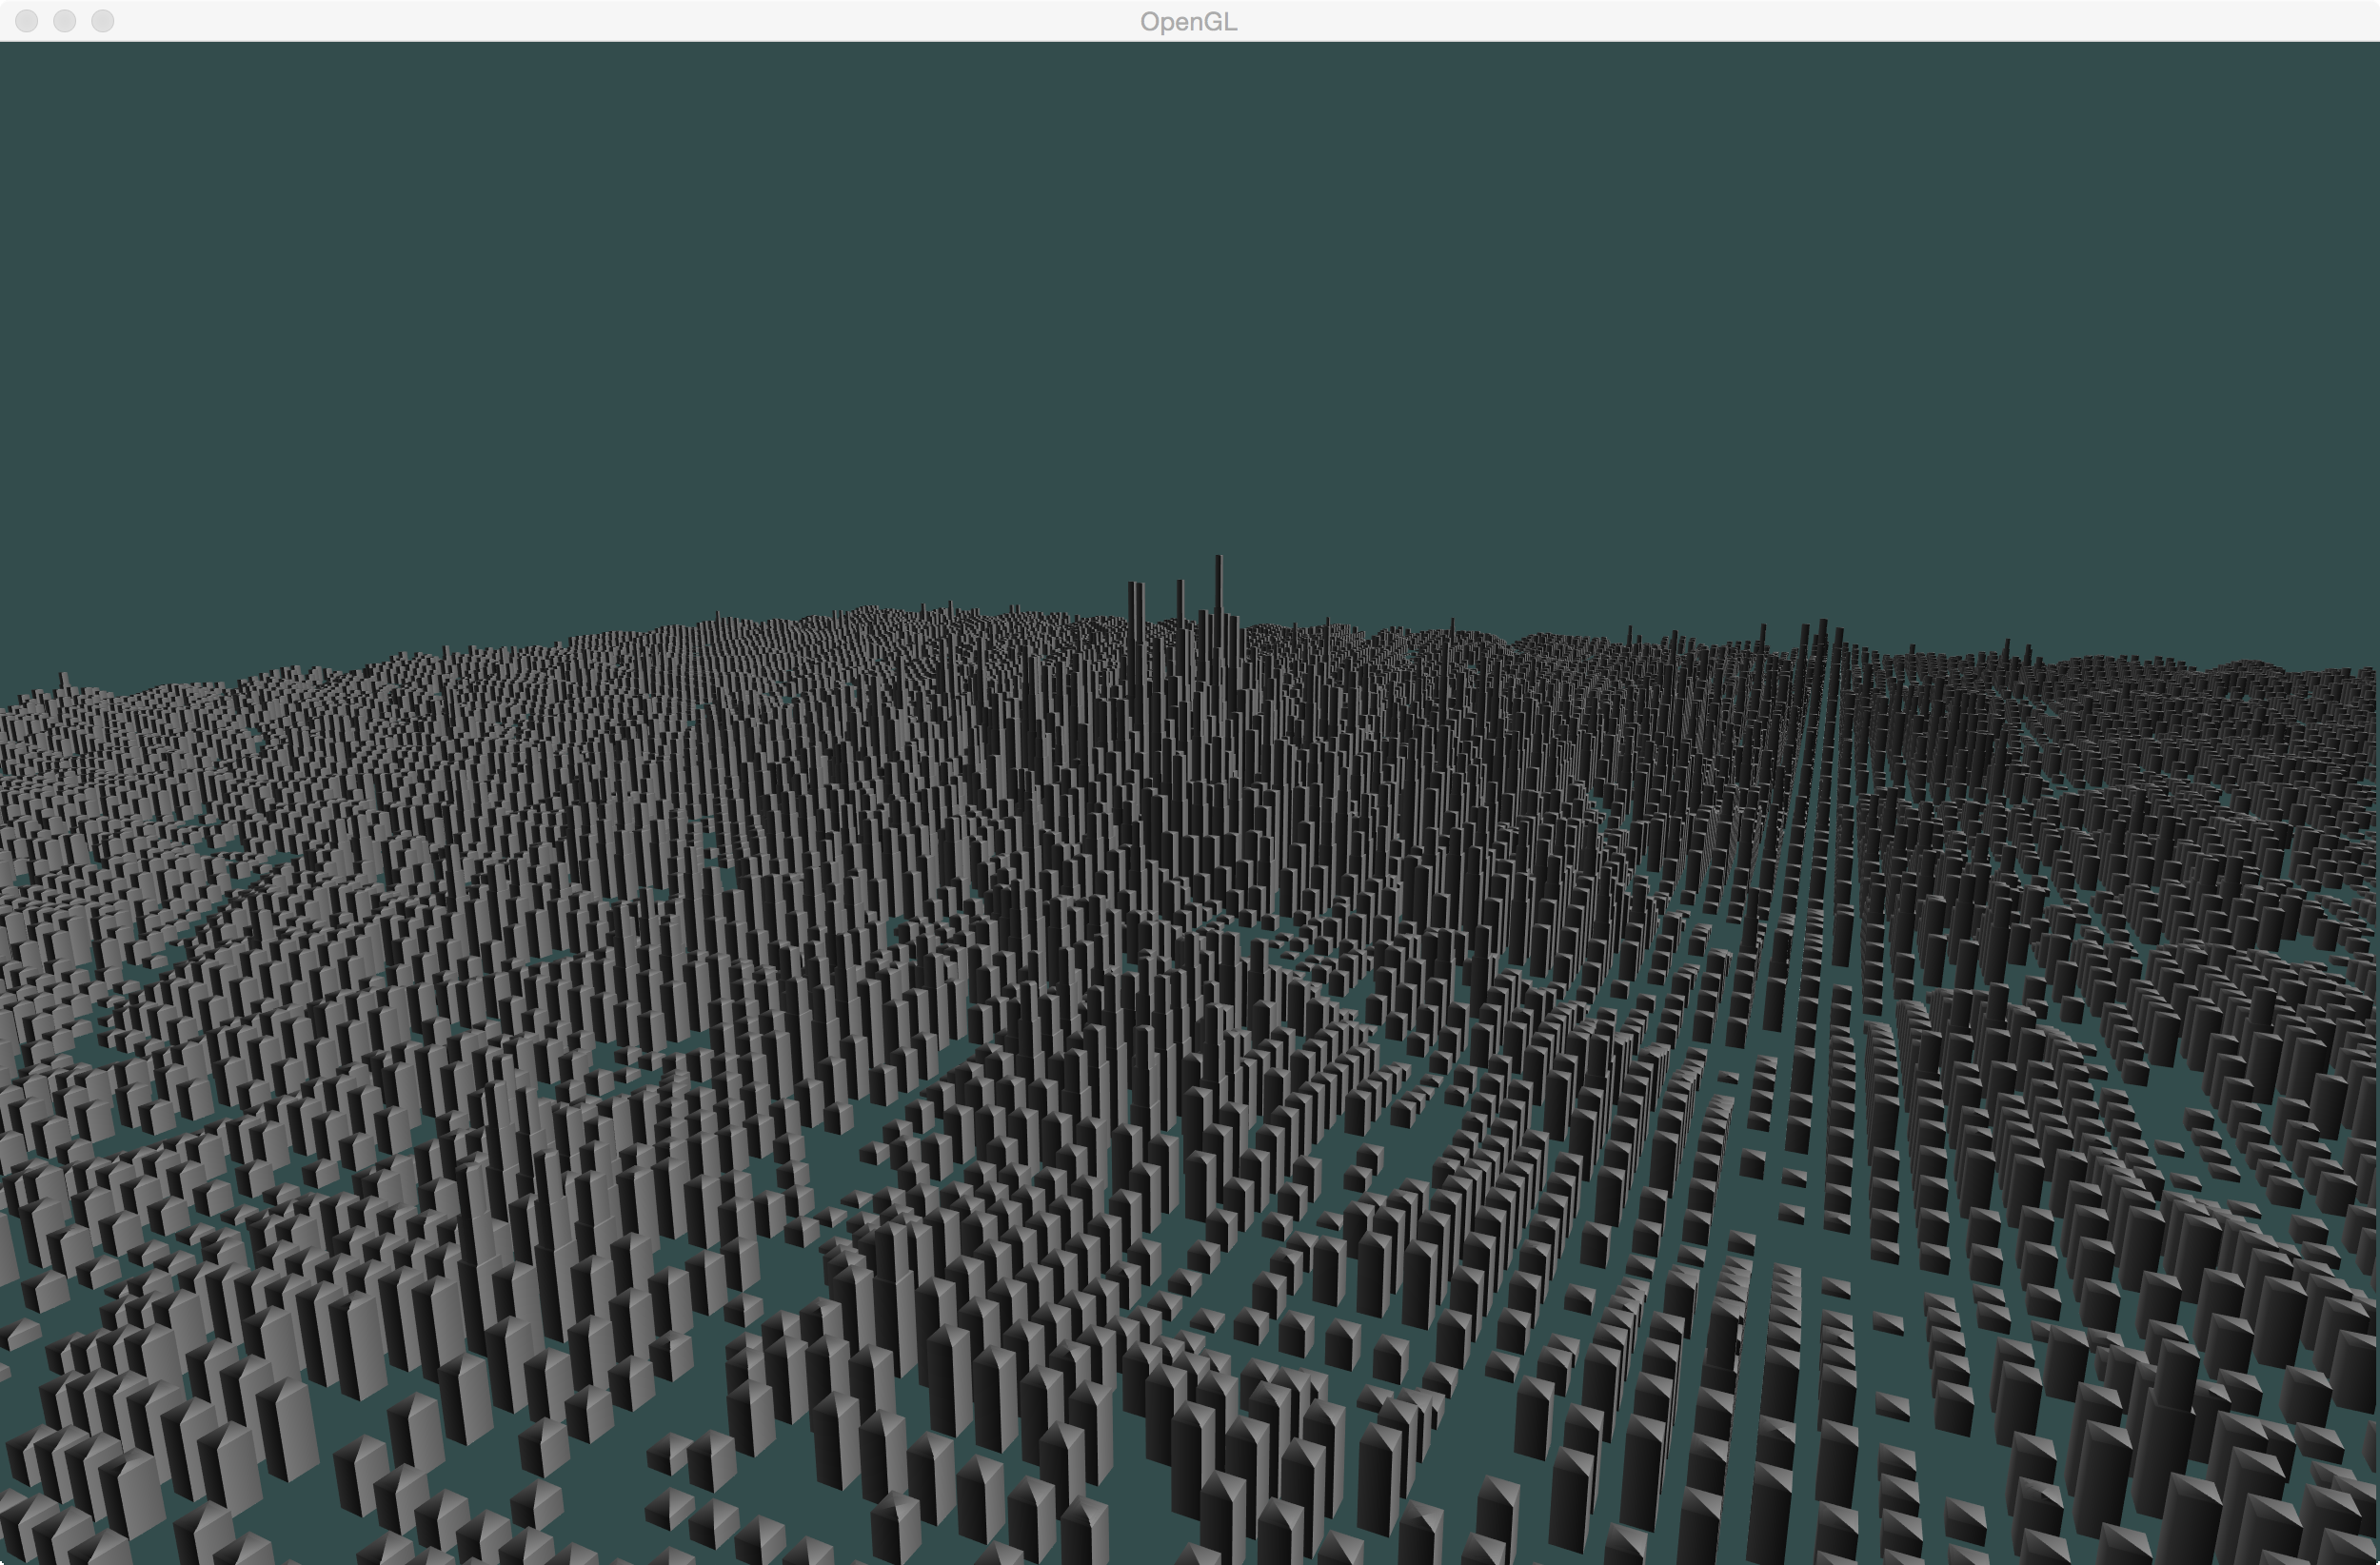
\includegraphics[width=0.95\textwidth]{img/Solution/City2-100*100.png}
	\caption{City Example}
	\label{fig:pic1}
\end{figure}



% section architecture (end)
